\documentclass{beamer}
\usepackage[utf8]{inputenc}
\usepackage[francais]{babel} 
\usepackage{graphicx} 
\usepackage{textcomp}
\usepackage{latexsym}
\usepackage{amssymb}
\usepackage{enumerate}
\usepackage{listings}
\usepackage{tikz}


\usetheme{Boadilla}
\setbeamertemplate{footline}
{
  \leavevmode%
      \hbox{%
        
   
\begin{beamercolorbox}[wd=.333333\paperwidth,ht=2.25ex,dp=1ex,center]{author in
head/foot}%
            \usebeamerfont{author in head/foot}
\thesection.\thesubsection~\insertsubsection
            \end{beamercolorbox}%
 
\begin{beamercolorbox}[wd=.333333\paperwidth,ht=2.25ex,dp=1ex,center]{title in
head/foot}%
            \usebeamerfont{title in head/foot}Smart Social Network
           \end{beamercolorbox}%
           
\begin{beamercolorbox}[wd=.333333\paperwidth,ht=2.25ex,dp=1ex,right]{date in
head/foot}%
            \usebeamerfont{date in
head/foot}\hspace*{2em}
        \insertframenumber{} / \inserttotalframenumber\hspace*{2ex} 
       \end{beamercolorbox}}%
          \vskip0pt%
}

\setbeamertemplate{blocks} [rounded] [shadow=false] 

\setbeamertemplate{navigation symbols}{
%     \insertslidenavigationsymbol
%         \insertframenavigationsymbol
%         \insertsubsectionnavigationsymbol
%         \insertsectionnavigationsymbol
%         \insertdocnavigationsymbol
%         \insertbackfindforwardnavigationsymbol
}

%\setbeamercolor{normal text}{fg=white,bg=black!90}
%\setbeamercolor{structure}{fg=white}
%
%\setbeamercolor{alerted text}{fg=red!85!black}
%
%\setbeamercolor{item projected}{use=item,fg=black,bg=item.fg!35}
%
%\setbeamercolor*{palette primary}{use=structure,fg=structure.fg}
%\setbeamercolor*{palette secondary}{use=structure,fg=structure.fg!95!black}
%\setbeamercolor*{palette tertiary}{use=structure,fg=structure.fg!90!black}
%\setbeamercolor*{palette quaternary}{use=structure,fg=structure.fg!95!black,bg=black!80}
%
%\setbeamercolor*{framesubtitle}{fg=white}
%
%\setbeamercolor*{block title}{parent=structure,bg=black!60}
%\setbeamercolor*{block body}{fg=black,bg=black!10}
%\setbeamercolor*{block title alerted}{parent=alerted text,bg=black!15}
%\setbeamercolor*{block title example}{parent=example text,bg=black!15}


\title{Smart Social Network}
\subtitle{Projet de Master 2 SSI}

\author{
    Zakaria \textsc{Addi},
    Baptiste \textsc{Dolbeau},\\
    Yicheng \textsc{Gao},
    Florian \textsc{Guilbert},\\
    Giovanni \textsc{Huet},
    Emmanuel \textsc{Mocquet},\\
    Maxence \textsc{Péchoux},
    Romain \textsc{Pignard}
}
\institute{Université de Rouen}

\AtBeginSection[]
{
    \begin{frame}
        \frametitle{Plan}
        \tableofcontents[currentsection,hideothersubsections]
    \end{frame}
}

\begin{document}

\begin{frame}
    \titlepage 
\end{frame}

\begin{frame}
    \frametitle{Plan}
    \tableofcontents[hideallsubsections]
\end{frame}

\section{Introduction}

\subsection{Présentation}
\begin{frame}
    \frametitle{Sujets}
    \begin{block}{SmartCard}
       Étude et mise en \oe{}uvre de solutions d’authentification et de signature 
       par cartes à puce. (Mme \textsc{Bardet})
    \end{block}
    \begin{block}{Secure Social Network}
       Solutions cryptographiques pour les réseaux sociaux. (M. \textsc{Otmani})
    \end{block}
    \pause
    \begin{block}{Fusion des projets : Smart Social Network}
       Développer une solution cryptographique pour un réseau social en 
      utilisant une base cryptographique sûre (carte à puce). 
    \end{block}
\end{frame}

\subsection{Gestion de projet}
\begin{frame}
    \frametitle{Gestion de projet}
    \begin{block}{Organisation}
        \begin{itemize}
            \item deux groupes (SC et SSN);
            \item quatre itérations.
            \item réunion hebdomadaire avec les clients;
            \item documentations (STB, DAL, AdR, CdR, ...);
        \end{itemize}
    \end{block}
\end{frame}

\section{Carte à puce}

\subsection{Introduction}
\begin{frame}
\frametitle{Introduction}
\begin{block}{Besoins}
\begin{itemize}
\item Authentification forte
\item Contenir des informations confidentielles
\end{itemize}
\end{block}

\begin{exampleblock}{Technologies étudiées}
\begin{itemize}
\item Génération de nombres aléatoires
\item Chiffrement/Déchiffrement
\item Signature/Vérification
\item Code PIN/PUK
\item SoftCard
\end{itemize}
\end{exampleblock}

\end{frame}

\subsection{Java Card}
\begin{frame}
    \frametitle{Présentation}
    \begin{block}{Rappel sur la carte à puce}
        \begin{itemize}
            \item Dispose d'un processeur pour du traitement d'informations.
            \item Permet de stocker des données cachées.
            \item Assure l'authentification de l'utilisateur.
        \end{itemize}
    \end{block}
    \begin{block}{"Java Card" : qu'est-ce ?}
        \begin{itemize}
            \item Désigne la technologie permettant de développer
                des applets \og sécurisées \fg{} sur carte à puce.

            \item Mais c'est aussi une carte à puce : 
                \begin{itemize}
                    \item programmable 
                    \item multi-applications
                    \item interopérable
                \end{itemize}
        \end{itemize}
    \end{block}
\end{frame}

\begin{frame}[fragile]
    \frametitle{Abstraction}
    \begin{block}{L'API Java Card}
        \begin{itemize}
            \item Permet de s'abstraire de l'assembleur $\rightarrow$ Java
            \item Fournit un certain nombre d'objets : PIN, clefs RSA...
        \end{itemize}
    \end{block}
    \begin{block}{Exemple}
    
        \lstset{language=Java,basicstyle=\scriptsize,keywordstyle=\color{red}
            \bfseries,commentstyle=\color{blue}\textit,labelstyle=\tiny, frame=singe}
        \begin{lstlisting}
    // Nouveau PIN d'une taille de 2 octets, 
    // avec 3 tentatives.
    pin = new OwnerPIN((byte) 3, (byte) 2 );
    // Fixation d'un PIN aux octets 15 et 12 (i.e. 3852)
    pin.update(new byte[]{15,12}, (short) 0, (byte) 2);
        \end{lstlisting}
    \end{block}
\end{frame}

\begin{frame}
    \frametitle{Dialogues}
    \begin{block}{Les APDU}
        \begin{itemize}
            \item Application Protocol Data Unit.
            \item Unité de communication entre le lecteur et la carte.
        \end{itemize}
    \end{block}
    \begin{table}
        \begin{tabular}{|c|c|c|c|c|c|c|}
            \hline
            CLA & INS & P1 & P2 & Lc & Données & Le\\
            \hline
        \end{tabular}
        \newline
        \begin{tabular}{|c|c|}
            \hline
            Données & Status\\
            \hline
        \end{tabular}
        \caption{Structures d'une commande et d'une réponse}
    \end{table}
\end{frame}

\begin{frame}[fragile]
    \begin{block}{Exemple sans l'API Java Card}
        \begin{itemize}
            \item Commande : 0xB0 0x00 0x00 0x00 0x01 0x05
            \item Réponse : 0x02 0xf2 0x23 0x42 0xcf 0x90 0x00
        \end{itemize}
    \end{block}
    \begin{block}{Exemple avec l'API Java Card}
        \lstset{language=Java,basicstyle=\scriptsize,keywordstyle=\color{red}
            \bfseries,commentstyle=\color{blue}\textit,labelstyle=\tiny, frame=singe}
        \begin{lstlisting}
// Commande
ResponseAPDU r = channel.transmit(new CommandAPDU(
    (byte)0xB0, (byte) 0x00, (byte) 0x00, (byte) 0x00, 1));
// Partie donnees de la reponse 0x02 0xf2 0x23 0x42 0xcf
r.getData(); 
        \end{lstlisting}
    \end{block}
\end{frame}

\begin{frame}
    \frametitle{Principales contraintes}
    \begin{block}{Les limitations de l'API Java Card}
        \begin{itemize}
            \item types : boolean, byte, short, tableaux associés
            \item pas de \og garbage collector \fg{}
        \end{itemize}
    \end{block}
\end{frame}

\subsection{Les applications développées}
\begin{frame}
    \frametitle{Les applications développées}
    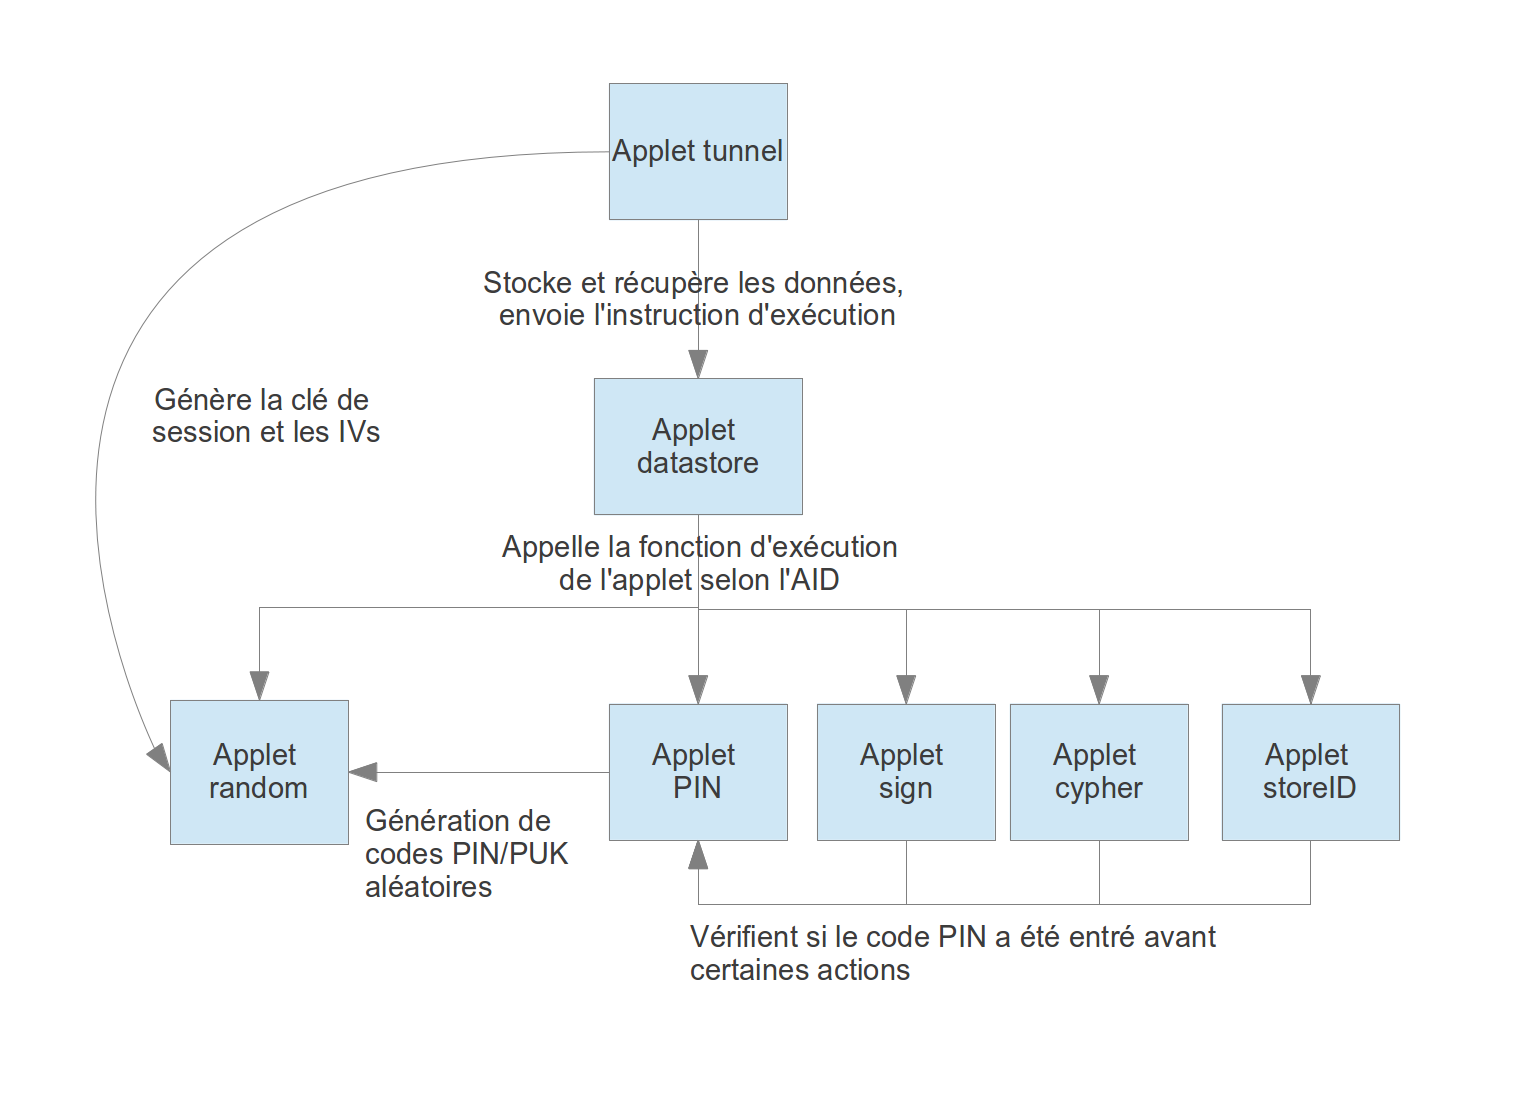
\includegraphics[width=10cm]{graphe_dep}
    \begin{block}{}
    \end{block}
\end{frame}

\subsection{L'aspect sécurité}
\begin{frame}
    \frametitle{L'aspect sécurité}
    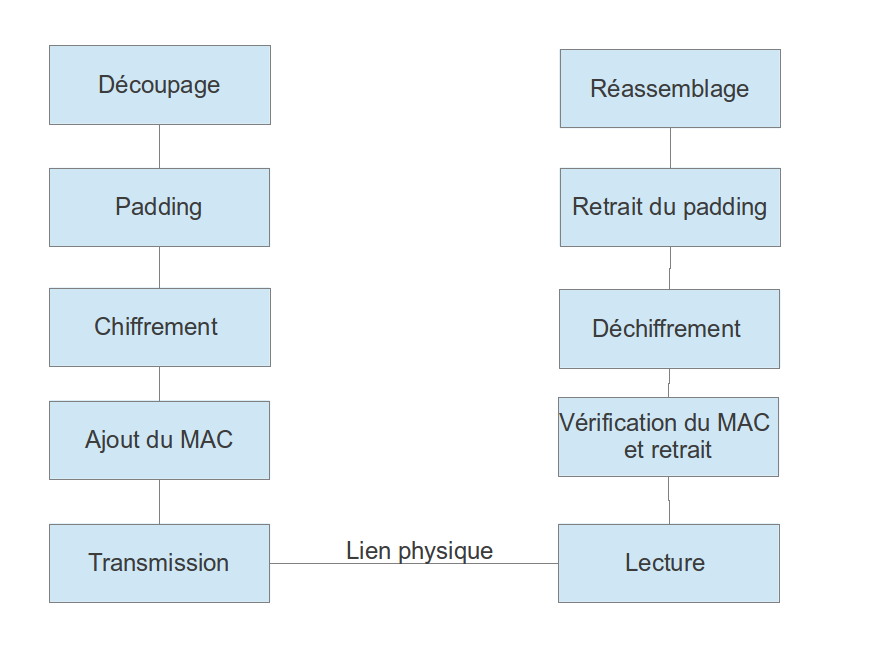
\includegraphics[width=9cm]{stack}
    % \begin{block}{}
    % \end{block}
\end{frame}

\subsection{Démonstration}
\begin{frame}
    \frametitle{Démonstration}
    \begin{block}{}
    \end{block}
\end{frame}

\subsection{SoftCard}
\begin{frame}
\frametitle{L'interface entre SSN et la carte}
    \frametitle{L'interface entre SSN et la carte}
    \begin{block}{Actuellement}
        \begin{itemize}
            \item Applications de chiffrement, déchiffrement, signature, stockage...
            \item Client testant ces applications.
        \end{itemize}
    \end{block}

    Mais par rapport à Facebook ?
\end{frame}

\begin{frame}
    \frametitle{L'interface entre SSN et la carte}
    \begin{block}{Un serveur vis-à-vis de SSN}
        \begin{itemize}
            \item Une entité (SoftCardServer) est instanciée et se met en
                attente de connexions.
            \item Pour chaque requête reçue, une action est transmise
                à une seconde entité : SoftCard.
            \item SoftCardServer renvoie le résultat de SoftCard au client.
        \end{itemize}
    \end{block}
    \begin{block}{Un client vis-à-vis de la carte}
        \begin{itemize}
            \item Une unique instance de SoftCard se connecte au lecteur puis à
                la carte.
            \item Différentes méthodes permettent de déchiffrer, signer...
            \item Pour certaines, sensibles, la carte devra être déverrouillée.
        \end{itemize}
    \end{block}
\end{frame}

\section{Une protection contre Facebook}

\subsection{Les besoins et exigences}
\begin{frame}
    \frametitle{Les besoins et exigences}
    \begin{block}{}

        Protection des données utilisateur vis-à-vis de tiers

        Authentification forte par carte à puce 
    \end{block}
\end{frame}

\subsection{Présentation des composants}
\begin{frame}
    \frametitle{Présentation des composants}
    %\begin{block}{ }
    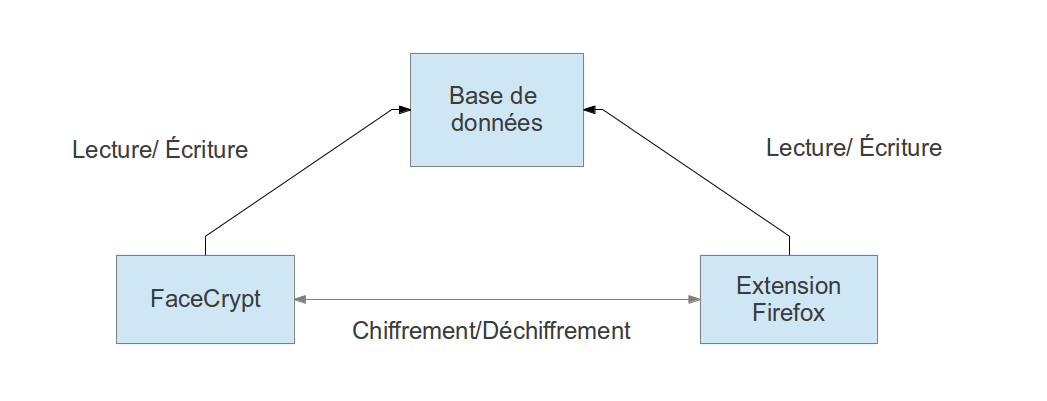
\includegraphics[width=12cm]{schema_zako}
    % \end{block}
\end{frame}


\begin{frame}
    \frametitle{Base de données}
    \begin{block}{Moteur SQLite }
        Base de données locale

        Accessible depuis Java et l'extension 
    \end{block}
    \begin{block}{Stockage des liens d'amitié dans la base}
        Listes d'amis


        Clés publiques


    \end{block}
\end{frame}


\subsection{Facecrypt}
\begin{frame}
    \frametitle{La communication}
    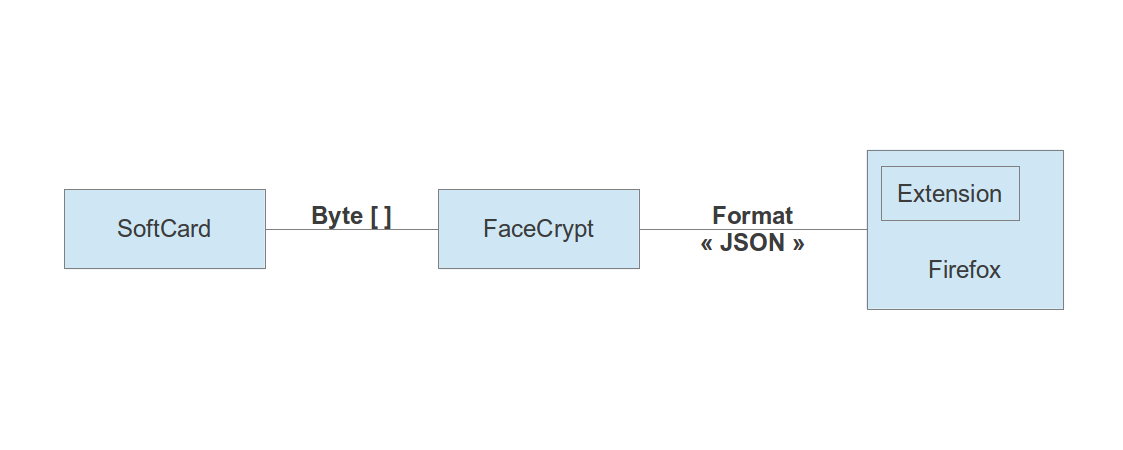
\includegraphics[width=11cm]{schema_dolby}
\end{frame}

\begin{frame}
    \frametitle{Composition}
    \begin{block}{Six classes java}
        \begin{itemize}
            \item ASymCypher
            \item SymCypher
            \item ServerSSL
            \item Client
            \item Dataprocess
            \item CacheManager
        \end{itemize}
    \end{block}
\end{frame}

\begin{frame}
    \frametitle{Exemple de cycle}

    \begin{itemize}
        \item Received from Facecrypt : \{"action":"getID"\}
        \item Sent to Softcard : 47
        \item Received from Softcard : $\underbrace{666f6f2e6261722e33333434393133}_{\textrm{login}} 20 \underbrace{726f6f74726f6f74}_{\textrm{password}}$
        \item Sent to Facecrypt : \{"action":"getID" ,"login":"foo.bar.3344913","firstConnection":false, "pass":"rootroot"\}
    \end{itemize}

    % \end{block}
\end{frame}

\subsection{SSNExt}

\begin{frame}
    \frametitle{Les extensions Firefox}
    \begin{block}{Javascript} 
    Langage de script orienté objet
    \end{block}
    \begin{block}{Add-on SDK Mozilla}
    Environnement de développement pour les extensions Firefox
    \end{block}
    \begin{block}{Add-on Builder}
    Plateforme en ligne d'utilisation du SDK, permet le \emph{versionning}
    \end{block}
\end{frame}

\begin{frame}
    \frametitle{Schéma de fonctionnement}
    \begin{center}
    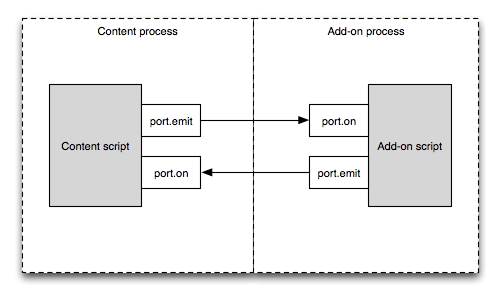
\includegraphics[width=11cm]{content-scripting-events.png}
    \end{center}
\end{frame}

\begin{frame}
    \frametitle{Modification du DOM}
    \begin{block}{Apparence fidèle} 
    Conservation du \emph{Look and Feel}
    \end{block}
    \begin{block}{Ajouts d'éléments}
        \begin{itemize}
            \item{Boutons de chiffrement, déchiffrement, 
            gestion des clefs...}
            \item{Listes d'amis, liens de modifications...}
        \end{itemize}
    \end{block}
\end{frame}

\begin{frame}
    \frametitle{Communication sécurisée}
    \begin{block}{Tunnel SSL}
    Communication via sockets, utilisation PKCS\#12 de Firefox,
    utilisation librairies NSS de Mozilla
    \end{block}
    \begin{block}{Gestion des évènements}
    Plusieurs types d'évènements au niveau des librairies
    \end{block}
\end{frame}

\begin{frame}
    \frametitle{Interaction avec la Base de Données}
    \begin{block}{Manipulation des fichiers}
    Création d'une instance de la Base de Données à la reception du pseudo,
    module FileUtils
    \end{block}
    \begin{block}{Cas d'utilisations}
    Synchronisation clefs publiques, ajout/modification/suppression
    de listes d'amis
    \end{block}
\end{frame}

\section{Démonstration}
\begin{frame}
    \frametitle{Démonstration}
    \begin{center}
    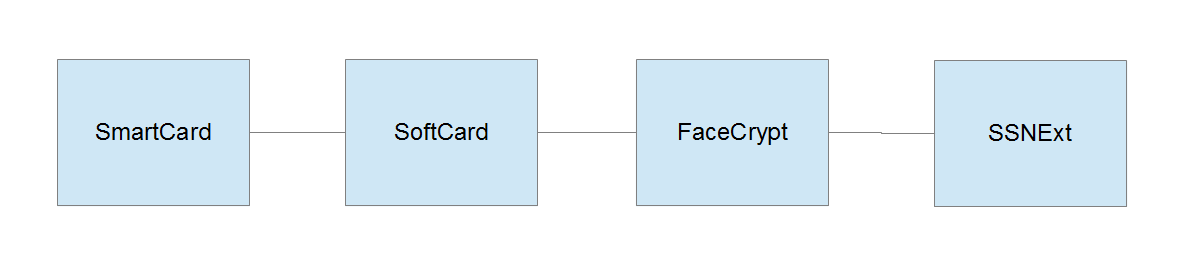
\includegraphics[width=11cm]{all.png}
    \end{center}
\end{frame}

\section{Conclusion}
\subsection{Difficultés rencontrées}
\begin{frame}
    \frametitle{Conclusion}
    \begin{alertblock}{Difficultés rencontrées}
        \begin{itemize}
            \item SmartCard : 
                \begin{itemize}
                    \item taille des données; % limitées dans les APDUs (256)
                    \item communications sécurisées entre la carte à puce et l'application
                        cliente;
                    \item installations des lecteurs;
                    \item stockage \og caché \fg{}; % vérifier que c'est vraiment caché
                    \item algorithmes implantés sur la carte;
                \end{itemize}
            \item Secure Social Network : 
                \begin{itemize}
                    \item manipulation de la page Facebook;
                    \item communications sécurisées entre SSNExt et FaceCrypt;
                    \item fonctionnement d'une extension.
                \end{itemize}
        \end{itemize}
    \end{alertblock}
\end{frame}

\subsection{Améliorations possibles}

\begin{frame}
    \frametitle{Conclusion}
    \begin{block}{Améliorations possibles}
        \begin{itemize}
            \item SmartCard : 
                \begin{itemize}
                    \item IHM pour entrer le code PIN; % => démon
                    \item Gestion de l'arrachage de la carte; % lors d'une opération, 
                        % la carte plante le cliente, débranchage, rebranchage avant une opération est géré.
                    \item One Time Password;
                    \item prendre en compte les attaques (canaux cachés);
                \end{itemize}
            \item Secure Social Network : 
                \begin{itemize}
                    \item finalisation pour mise en production;
                    \item abstraction du réseau social pour l'extension;
                    \item étudier le tatouage d'images.
                \end{itemize}
        \end{itemize}
    \end{block}
\end{frame}

\subsection{Apports}
\begin{frame}
    \frametitle{Conclusion}
    \begin{block}{Ce que cela nous a apporté}
        \begin{itemize}
            \item SmartCard : 
                \begin{itemize}
                    \item manipulation d'une carte à puce;
                \end{itemize}
            \item Secure Social Network : 
                \begin{itemize}
                    \item gestion d'une communication sécurisées entre plusieurs
                        composants;
                \end{itemize}
            \item utilisation concrête de la cryptographie;
            \item travail en équipe.
        \end{itemize}
    \end{block}
\end{frame}

\begin{frame}
\begin{center}Merci pour votre attention.\\[2cm]
          Des questions ?\end{center}
\end{frame}

\end{document}
